\documentclass[12pt,a4paper]{book}
\usepackage{lmodern}
\usepackage{amssymb,amsmath}
\usepackage{ifxetex,ifluatex}
\usepackage{fixltx2e} % provides \textsubscript
\ifnum 0\ifxetex 1\fi\ifluatex 1\fi=0 % if pdftex
  \usepackage[T1]{fontenc}
  \usepackage[utf8]{inputenc}
\else % if luatex or xelatex
  \ifxetex
    \usepackage{mathspec}
  \else
    \usepackage{fontspec}
  \fi
  \defaultfontfeatures{Ligatures=TeX,Scale=MatchLowercase}
\fi
% use upquote if available, for straight quotes in verbatim environments
\IfFileExists{upquote.sty}{\usepackage{upquote}}{}
% use microtype if available
\IfFileExists{microtype.sty}{%
\usepackage{microtype}
\UseMicrotypeSet[protrusion]{basicmath} % disable protrusion for tt fonts
}{}
\usepackage[margin=2cm]{geometry}
\usepackage{hyperref}
\PassOptionsToPackage{usenames,dvipsnames}{color} % color is loaded by hyperref
\hypersetup{unicode=true,
            pdftitle={Notes on a design of a simple spatial sampling method (S3M) for assessing coverage of health and nutrition programmes in Liberia},
            pdfauthor={Valid International},
            colorlinks=true,
            linkcolor=Maroon,
            citecolor=Blue,
            urlcolor=Blue,
            breaklinks=true}
\urlstyle{same}  % don't use monospace font for urls
\usepackage{natbib}
\bibliographystyle{apalike}
\usepackage{longtable,booktabs}
\usepackage{graphicx,grffile}
\makeatletter
\def\maxwidth{\ifdim\Gin@nat@width>\linewidth\linewidth\else\Gin@nat@width\fi}
\def\maxheight{\ifdim\Gin@nat@height>\textheight\textheight\else\Gin@nat@height\fi}
\makeatother
% Scale images if necessary, so that they will not overflow the page
% margins by default, and it is still possible to overwrite the defaults
% using explicit options in \includegraphics[width, height, ...]{}
\setkeys{Gin}{width=\maxwidth,height=\maxheight,keepaspectratio}
\IfFileExists{parskip.sty}{%
\usepackage{parskip}
}{% else
\setlength{\parindent}{0pt}
\setlength{\parskip}{6pt plus 2pt minus 1pt}
}
\setlength{\emergencystretch}{3em}  % prevent overfull lines
\providecommand{\tightlist}{%
  \setlength{\itemsep}{0pt}\setlength{\parskip}{0pt}}
\setcounter{secnumdepth}{5}
% Redefines (sub)paragraphs to behave more like sections
\ifx\paragraph\undefined\else
\let\oldparagraph\paragraph
\renewcommand{\paragraph}[1]{\oldparagraph{#1}\mbox{}}
\fi
\ifx\subparagraph\undefined\else
\let\oldsubparagraph\subparagraph
\renewcommand{\subparagraph}[1]{\oldsubparagraph{#1}\mbox{}}
\fi

%%% Use protect on footnotes to avoid problems with footnotes in titles
\let\rmarkdownfootnote\footnote%
\def\footnote{\protect\rmarkdownfootnote}

%%% Change title format to be more compact
\usepackage{titling}

% Create subtitle command for use in maketitle
\newcommand{\subtitle}[1]{
  \posttitle{
    \begin{center}\large#1\end{center}
    }
}

\setlength{\droptitle}{-2em}
  \title{Notes on a design of a simple spatial sampling method (S3M) for
assessing coverage of health and nutrition programmes in Liberia}
  \pretitle{\vspace{\droptitle}\centering\huge}
  \posttitle{\par}
  \author{Valid International}
  \preauthor{\centering\large\emph}
  \postauthor{\par}
  \predate{\centering\large\emph}
  \postdate{\par}
  \date{2018-06-22}

\usepackage{booktabs}
\usepackage{color}
\usepackage{tcolorbox}
\usepackage{float}
\usepackage{setspace}

\onehalfspacing

\graphicspath{ {icons/} }

\newenvironment{rmdremind}
  {\begin{tcolorbox}[width=\textwidth, 
                     colback = {white}, 
                     title = {\textbf{Remember}}, 
                     colbacktitle = lightgray,
                     coltitle = black]
  \begin{includegraphics}[scale = 1]{remind.png}
  \begin{itemize}}
  {\end{itemize}
  \end{includegraphics}
  \end{tcolorbox}}

\newenvironment{rmdnote}
  {\begin{tcolorbox}[width=\textwidth, 
                     colback = {white}, 
                     title = {\textbf{Note}}, 
                     colbacktitle = lightgray,
                     coltitle = black]
  \begin{includegraphics}[scale = 1]{pencil.png}}
  {\end{includegraphics}
  \end{tcolorbox}}
  
\newenvironment{rmdcalc}
  {\begin{tcolorbox}[width=\textwidth, 
                     colback = {white}, 
                     title = {\textbf{Calculations}}, 
                     colbacktitle = lightgray,
                     coltitle = black]
  \begin{includegraphics}[scale = 1]{pencil.png}}
  {\end{includegraphics}
  \end{tcolorbox}}
  
\newenvironment{rmdexercise}
  {\begin{tcolorbox}[width=\textwidth, 
                     colback = {white}, 
                     title = {\textbf{Exercise}}, 
                     colbacktitle = lightgray,
                     coltitle = black]
  \begin{includegraphics}[scale = 1]{exercise.png}}
  {\end{includegraphics}
  \end{tcolorbox}}
  
\newenvironment{rmdbox}
  {\begin{tcolorbox}[width=\textwidth, 
                     colback = {white}, 
                     title = {\textbf{Exercise}}, 
                     colbacktitle = lightgray,
                     coltitle = black]
  \begin{includegraphics}[scale = 1]{pencil.png}}
  {\end{includegraphics}
  \end{tcolorbox}}
  
\newenvironment{rmdinfo}
  {\begin{tcolorbox}[width=\textwidth, 
                     colback = {white}, 
                     title = {\textbf{Info}}, 
                     colbacktitle = lightgray,
                     coltitle = black]
  \begin{includegraphics}[scale = 1]{info.png}}
  {\end{includegraphics}
  \end{tcolorbox}}  
  
\newenvironment{rmdwarning}
  {\begin{tcolorbox}[width=\textwidth, 
                     colback = {white}, 
                     title = {\textbf{Warning}}, 
                     colbacktitle = lightgray,
                     coltitle = black]
  \begin{includegraphics}[scale = 1]{warning.png}}
  {\end{includegraphics}
  \end{tcolorbox}}

\newenvironment{rmddownload}
  {\begin{tcolorbox}[width=\textwidth, 
                     colback = {white}, 
                     title = {\textbf{Download}}, 
                     colbacktitle = lightgray,
                     coltitle = black]
  \begin{includegraphics}[scale = 1]{download.png}}
  {\end{includegraphics}
  \end{tcolorbox}}

\usepackage{amsthm}
\newtheorem{theorem}{Theorem}[chapter]
\newtheorem{lemma}{Lemma}[chapter]
\theoremstyle{definition}
\newtheorem{definition}{Definition}[chapter]
\newtheorem{corollary}{Corollary}[chapter]
\newtheorem{proposition}{Proposition}[chapter]
\theoremstyle{definition}
\newtheorem{example}{Example}[chapter]
\theoremstyle{definition}
\newtheorem{exercise}{Exercise}[chapter]
\theoremstyle{remark}
\newtheorem*{remark}{Remark}
\newtheorem*{solution}{Solution}
\let\BeginKnitrBlock\begin \let\EndKnitrBlock\end
\begin{document}
\maketitle

{
\hypersetup{linkcolor=black}
\setcounter{tocdepth}{1}
\tableofcontents
}
\hypertarget{simple-spatial-sampling-method-s3m}{%
\chapter*{Simple Spatial Sampling Method
(S3M)}\label{simple-spatial-sampling-method-s3m}}
\addcontentsline{toc}{chapter}{Simple Spatial Sampling Method (S3M)}

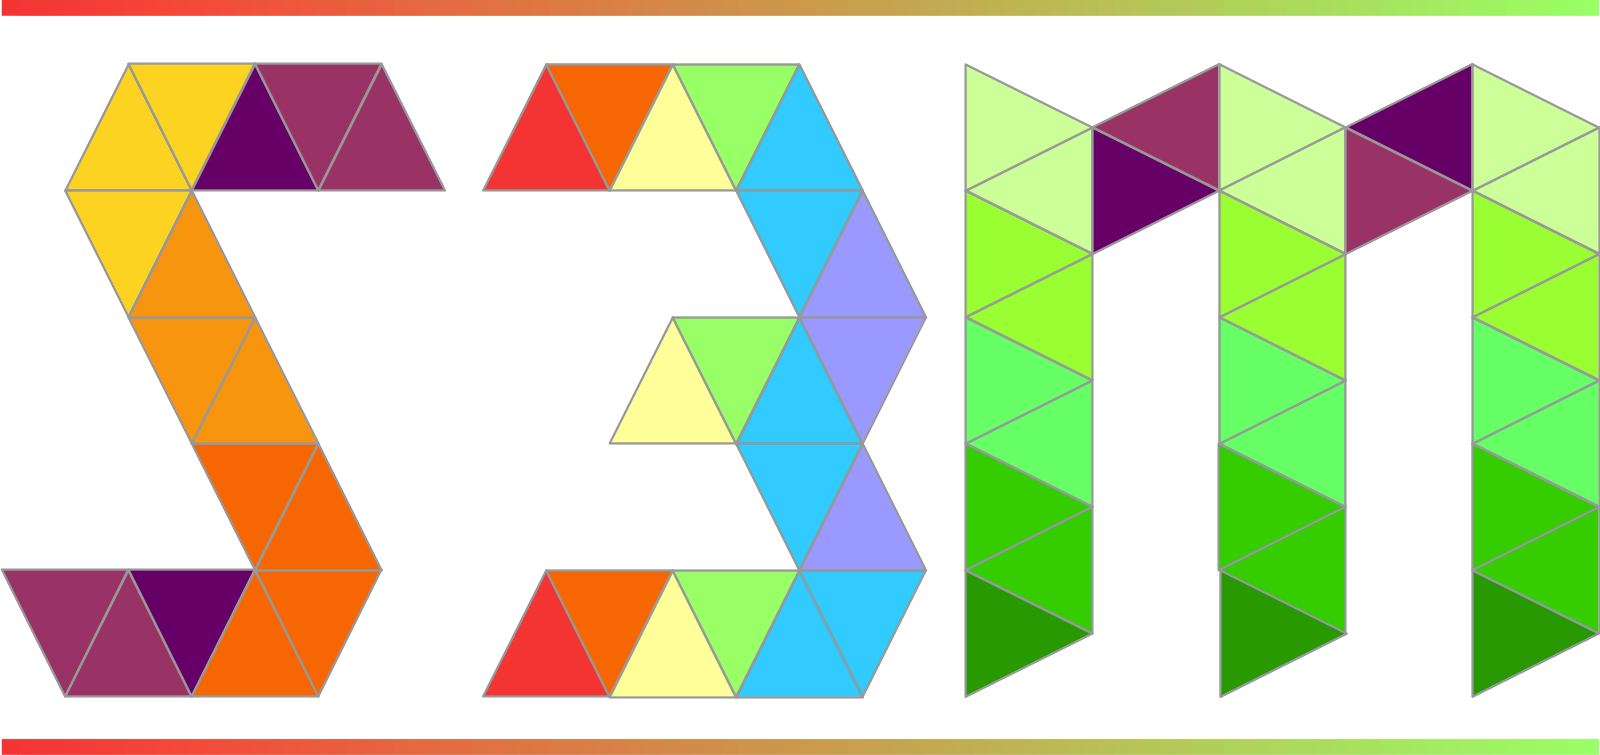
\includegraphics{figures/s3mlogo.png}

\hypertarget{introduction}{%
\chapter{Introduction}\label{introduction}}

The Simple Spatial Survey Method (S3M) was developed from the CSAS
coverage survey method as a response to the widespread adoption of
community management of acute malnutrition (CMAM) by ministries of
health. Large-scale programs need a large-scale survey method and S3M
was developed to meet that need.

S3M was designed to :

\begin{itemize}
\item
  Be simple enough for MoH, NGO, and UNO personnel without specialist
  statistical training to perform.
\item
  Provide a general survey method. S3M can be used to survey and map :
\item
  Need for and coverage of selective-entry programs such as CMAM and
  TSFP as well as universal programs such as EPI, GMP, GFD (general
  ration), and ``blanket'' SFP over wide areas.
\item
  Levels of indicators such as those for IYCF, WASH, and period
  prevalence / cumulative prevalence of ARI, fever, and diarrhoea over
  wide areas.
\end{itemize}

This document concentrates on using S3M to assess the need for and
coverage of a variety of selective-entry feeding programs. The
indicators discussed in this manual are:

\begin{itemize}
\item
  Therapeutic feeding (OTP and TSFP) programs :
\item
  Prevalence of SAM and coverage of treatment of SAM in children aged
  between 6 and 59 months.
\item
  Prevalence of MAM and coverage of treatment of MAM in children aged
  between 6 and 59 months.
\item
  Prevalence of MAM and treatment of MAM and in pregnant and lactating
  women (PLWs).
\item
  Food-based prevention of malnutrition (FBPM) programs :
\item
  Prevalence of need for and coverage of food-based prevention of
  malnutrition in younger children at risk of developing MAM and SAM.
\item
  Prevalence of need for and coverage of food-based prevention of
  malnutrition in pregnant and lactating women (PLWs) at risk of
  developing MAM and SAM.
\item
  Coverage of screening for all of the above programs.
\item
  Coverage of Behaviour Change Communication (BCC) programs focussing on
  maternal and child health and nutrition to all principal carers of
  children (usually their mothers) and all PLWs.
\end{itemize}

\hypertarget{sample}{%
\chapter{The survey sample}\label{sample}}

The survey method described here uses a two-stage sample:

\begin{itemize}
\item
  \textbf{First-stage:} We take an even (or near-even) spatial sample of
  communities from all of the communities in the survey area.
\item
  \textbf{Second-stage:} We take a sample of eligible individuals from
  each of the communities identified in the first stage of sampling.
\end{itemize}

Two-stage sampling is used in many survey methods. A typical example of
a survey method that uses a two- stage sample is the SMART method that
is commonly used for nutritional anthropometry surveys.

The main difference between the sample taken in S3M based surveys and in
SMART type surveys is that S3M based samples used a spatial sample in
the first stage whereas SMART type surveys use a proportional to
population size (PPS) sample.

The advantages of using a spatial first stage sample is that such a
sample allows us to identify where (and why) coverage is good, and where
(and why) coverage is poor. This information is essential to improving
program coverage and ensuring equitable access to services.

A spatial sample can be used to produce equivalent results to a
traditional proportional to population size (PPS) sample as is used in
(e.g.) SMART type surveys using a weighted analysis. This means that a
spatial sample can be made to act as a PPS sample. A PPS type sample
cannot, however, be made to act as a spatial sample.

\hypertarget{stage1}{%
\chapter{The first stage sample}\label{stage1}}

\hypertarget{step-1-find-a-map}{%
\section{Step 1: Find a map}\label{step-1-find-a-map}}

The first step in a S3M survey is to find a map of the survey area. A
map showing the locations of all towns and villages in the survey area
is essential. Try to find a map showing the locations of all towns and
villages in the survey area. You may need to update the map to take into
account migration and displacement.

For the coverage survey of 2 counties in Liberia, it will be practical
and useful to have:

\begin{itemize}
\tightlist
\item
  A small scale-map (a wide area map but with poor detail) of the entire
  survey area for each of the 2 counties. If the counties are contiguous
  (i.e., share borders with each other), the small scale map can be of
  the two counties together. This map does not need to show the location
  of all towns and villages in the survey area but it gives a general
  idea of where the 2 counties are located and main towns and locations
  and roads. Figure \ref{fig:smallScaleMap} is a small scale map of
  Liberia showing counties, roads and main towns and locations. Figure
  \ref{fig:smallScaleMapCounty} is a small scale map of two counties
  showing all the districts within the county, roads and main towns and
  locations.
\end{itemize}

\newpage

\begin{figure}[H]

{\centering 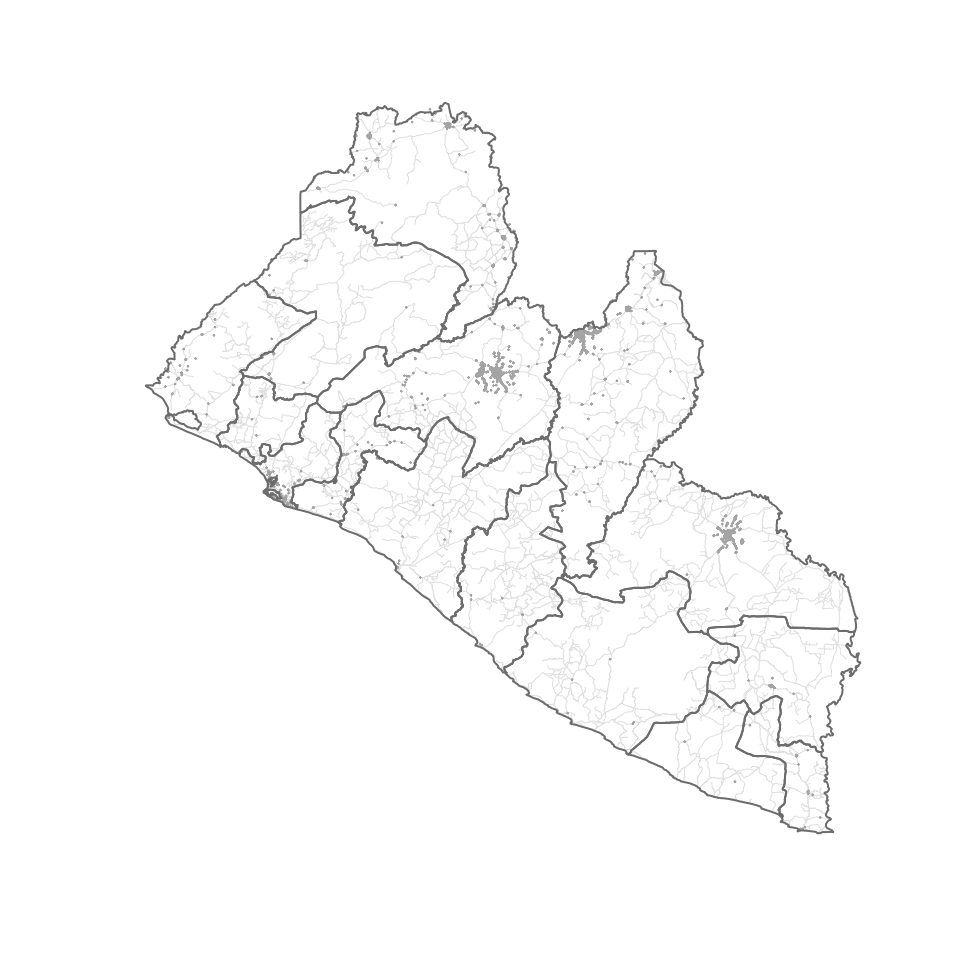
\includegraphics{figures/smallScaleMap-1} 

}

\caption{Small scale map of Liberia showing counties, roads and points of interest}\label{fig:smallScaleMap}
\end{figure}\newpage

\begin{figure}[H]

{\centering 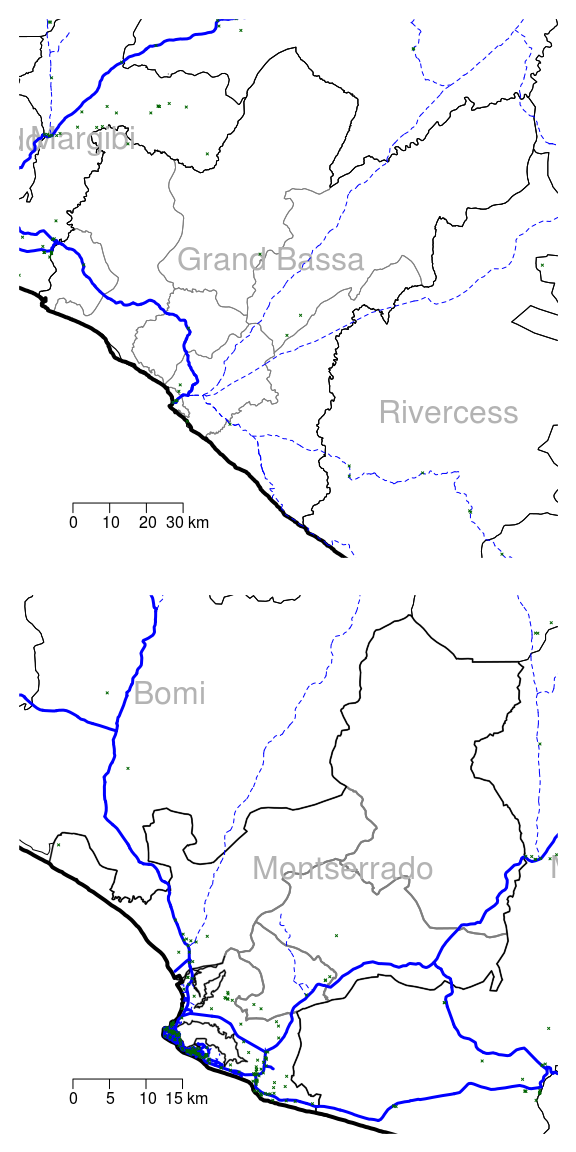
\includegraphics{figures/smallScaleMapCounty-1} 

}

\caption{Small scale map of two counties in Liberia showing all districts, roads and points of interest}\label{fig:smallScaleMapCounty}
\end{figure}\newpage

\begin{itemize}
\tightlist
\item
  A collection of larger scale maps (a small area map but with good
  detail) of each of the selected counties and each of the districts
  within those counties in Liberia. Figure \ref{fig:largeScaleMapCounty}
  is a large scale map of Montserrado county showing all districts,
  roads and all settlements. Figure \ref{fig:largeScaleMapDistricts} is
  a collection of large scale maps of each of the districts of
  Montserrado country showing all roads and all settlements.
\end{itemize}

~

\begin{figure}[H]

{\centering 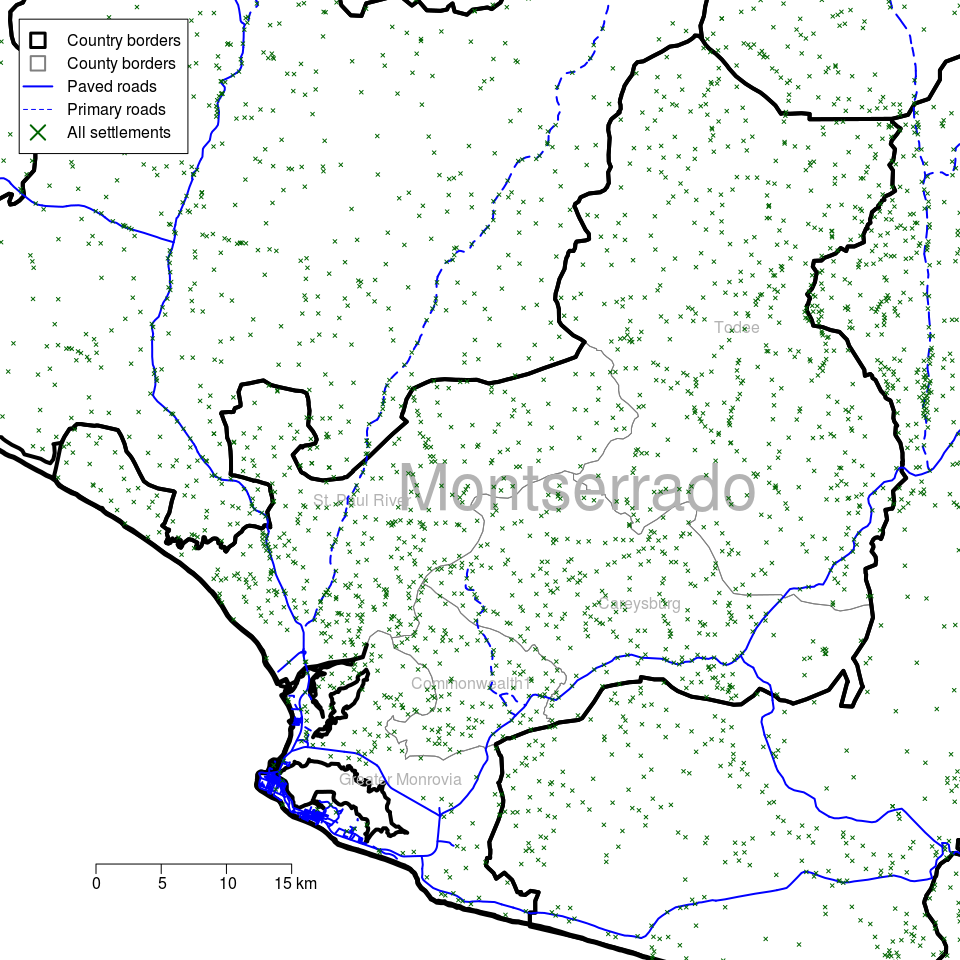
\includegraphics{figures/largeScaleMapCounty-1} 

}

\caption{Large scale map of Montserrado county in Liberia showing all districts, roads and all settlements (towns, villages)}\label{fig:largeScaleMapCounty}
\end{figure}

\newpage

\begin{figure}[H]

{\centering 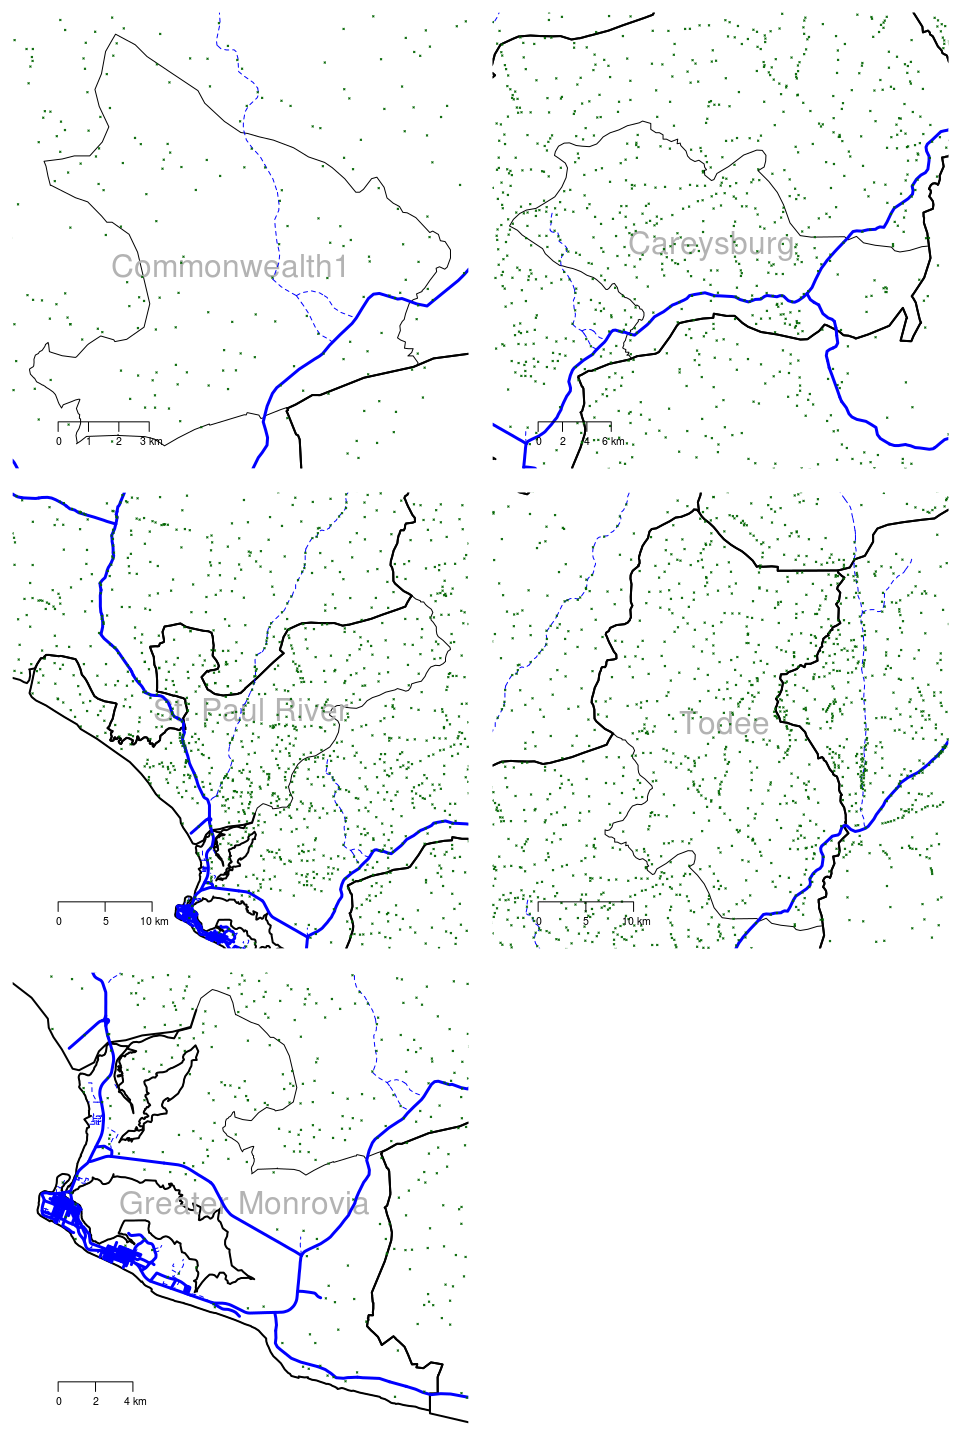
\includegraphics{figures/largeScaleMapDistricts-1} 

}

\caption{Large scale maps of 5 districts of Montserrado county in Liberia showing roads and all settlements (towns, villages)}\label{fig:largeScaleMapDistricts}
\end{figure}

\newpage

The small-scale maps in Figures \ref{fig:smallScaleMap} and
\ref{fig:smallScaleMapCounty} will be useful for identifying initial
sampling locations.

The large-scale maps in Figures \ref{fig:largeScaleMapCounty} and
\ref{fig:largeScaleMapDistricts} will be useful for identifying the
precise location of sampling points and for selecting the communities to
be sampled.

\newpage

\hypertarget{step-2-decide-the-area-to-be-represented-by-each-sampling-point}{%
\section{Step 2: Decide the area to be represented by each sampling
point}\label{step-2-decide-the-area-to-be-represented-by-each-sampling-point}}

The easiest way of thinking about this is as a function of the intended
maximum distance (\(d\)) of any community from the nearest sampling
point (see Figure \ref{fig:distance}.

~

\begin{figure}[H]

{\centering 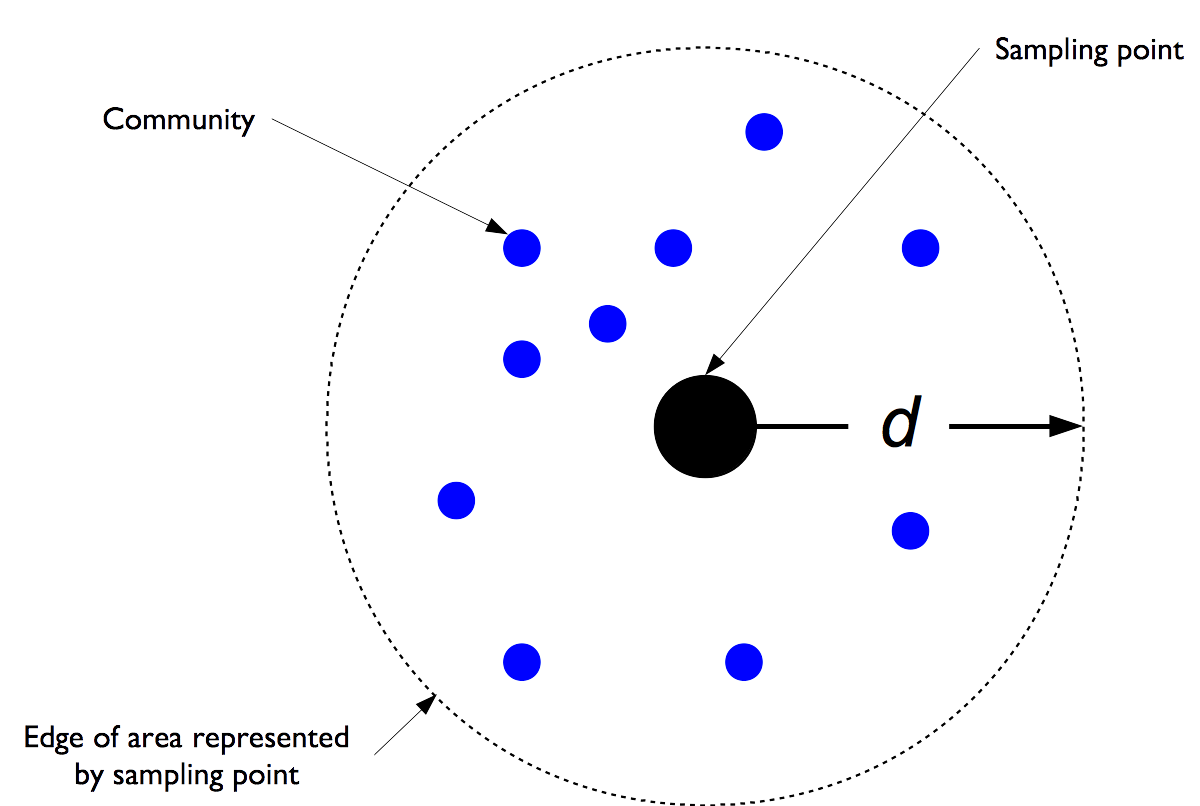
\includegraphics[width=16.67in]{figures/step2} 

}

\caption{Conceptual presentation of the area represented by each sampling point}\label{fig:distance}
\end{figure}

~

There are other ways of thinking about \(d\). These are:

\begin{itemize}
\tightlist
\item
  \textbf{The area of each triangular tile}: This can be calculated
  using the formula:
\end{itemize}

\[ A ~ = ~ \tan30^ \circ ~ \times ~ \frac{9}{4} ~ d ^ 2 \]

For \(d ~ = ~ 10 ~ \text{km}\) the area of each triangular tile will be
about:

\[ A ~ = ~ \tan30^ \circ ~ \times ~ \frac{9}{4} ~ d ^ 2 ~ \approx ~ 1.3 ~ \times ~ 100 ~ = ~ 130 ~ \text{km} ^ 2 \]

\begin{itemize}
\tightlist
\item
  \textbf{Practicability}: Most of the time spent in the field when
  doing a survey will be in travelling to and from sampling points.
  Having many sampling points can make for an expensive and / or lengthy
  survey. If you know how many sampling points that you can afford to
  take (\(m\)) then you can make a \textbf{very approximate} estimate of
  a suitable value for d using the following \emph{rule-of-thumb}
  formula:
\end{itemize}

\[ d ~ \approx ~ \sqrt{\frac{\text{Program Area}}{m}} \]

The value of \(d\) calculated using this formula is approximate and
should be used as a starting point for a number of trial samples using
the procedure outlined below.

S3M surveys have been done using a wide range (i.e.~from
\(d ~ = ~ 8 ~ \text{km}\) to \(d ~ = ~ 33 ~ \text{km}\)) of values for
\(d\). A value for \(d\) of \(10 ~ \text{km}\) or \(12 ~ \text{km}\)
will probably be small enough in most circumstances.

\begin{longtable}[]{@{}cccc@{}}
\toprule
\begin{minipage}[b]{0.14\columnwidth}\centering
\textbf{Pair}\strut
\end{minipage} & \begin{minipage}[b]{0.20\columnwidth}\centering
\textbf{Distance}\strut
\end{minipage} & \begin{minipage}[b]{0.14\columnwidth}\centering
\textbf{Pair}\strut
\end{minipage} & \begin{minipage}[b]{0.20\columnwidth}\centering
\textbf{Distance}\strut
\end{minipage}\tabularnewline
\midrule
\endhead
\begin{minipage}[t]{0.14\columnwidth}\centering
1\strut
\end{minipage} & \begin{minipage}[t]{0.20\columnwidth}\centering
21 km\strut
\end{minipage} & \begin{minipage}[t]{0.14\columnwidth}\centering
13\strut
\end{minipage} & \begin{minipage}[t]{0.20\columnwidth}\centering
13 km\strut
\end{minipage}\tabularnewline
\begin{minipage}[t]{0.14\columnwidth}\centering
2\strut
\end{minipage} & \begin{minipage}[t]{0.20\columnwidth}\centering
14 km\strut
\end{minipage} & \begin{minipage}[t]{0.14\columnwidth}\centering
14\strut
\end{minipage} & \begin{minipage}[t]{0.20\columnwidth}\centering
11 km\strut
\end{minipage}\tabularnewline
\begin{minipage}[t]{0.14\columnwidth}\centering
3\strut
\end{minipage} & \begin{minipage}[t]{0.20\columnwidth}\centering
13 km\strut
\end{minipage} & \begin{minipage}[t]{0.14\columnwidth}\centering
15\strut
\end{minipage} & \begin{minipage}[t]{0.20\columnwidth}\centering
12 km\strut
\end{minipage}\tabularnewline
\begin{minipage}[t]{0.14\columnwidth}\centering
4\strut
\end{minipage} & \begin{minipage}[t]{0.20\columnwidth}\centering
17 km\strut
\end{minipage} & \begin{minipage}[t]{0.14\columnwidth}\centering
16\strut
\end{minipage} & \begin{minipage}[t]{0.20\columnwidth}\centering
15 km\strut
\end{minipage}\tabularnewline
\begin{minipage}[t]{0.14\columnwidth}\centering
5\strut
\end{minipage} & \begin{minipage}[t]{0.20\columnwidth}\centering
11 km\strut
\end{minipage} & \begin{minipage}[t]{0.14\columnwidth}\centering
17\strut
\end{minipage} & \begin{minipage}[t]{0.20\columnwidth}\centering
13 km\strut
\end{minipage}\tabularnewline
\begin{minipage}[t]{0.14\columnwidth}\centering
6\strut
\end{minipage} & \begin{minipage}[t]{0.20\columnwidth}\centering
14 km\strut
\end{minipage} & \begin{minipage}[t]{0.14\columnwidth}\centering
18\strut
\end{minipage} & \begin{minipage}[t]{0.20\columnwidth}\centering
16 km\strut
\end{minipage}\tabularnewline
\begin{minipage}[t]{0.14\columnwidth}\centering
7\strut
\end{minipage} & \begin{minipage}[t]{0.20\columnwidth}\centering
12 km\strut
\end{minipage} & \begin{minipage}[t]{0.14\columnwidth}\centering
19\strut
\end{minipage} & \begin{minipage}[t]{0.20\columnwidth}\centering
18 km\strut
\end{minipage}\tabularnewline
\begin{minipage}[t]{0.14\columnwidth}\centering
8\strut
\end{minipage} & \begin{minipage}[t]{0.20\columnwidth}\centering
15 km\strut
\end{minipage} & \begin{minipage}[t]{0.14\columnwidth}\centering
20\strut
\end{minipage} & \begin{minipage}[t]{0.20\columnwidth}\centering
13 km\strut
\end{minipage}\tabularnewline
\begin{minipage}[t]{0.14\columnwidth}\centering
9\strut
\end{minipage} & \begin{minipage}[t]{0.20\columnwidth}\centering
16 km\strut
\end{minipage} & \begin{minipage}[t]{0.14\columnwidth}\centering
21\strut
\end{minipage} & \begin{minipage}[t]{0.20\columnwidth}\centering
8 km\strut
\end{minipage}\tabularnewline
\begin{minipage}[t]{0.14\columnwidth}\centering
10\strut
\end{minipage} & \begin{minipage}[t]{0.20\columnwidth}\centering
12 km\strut
\end{minipage} & \begin{minipage}[t]{0.14\columnwidth}\centering
22\strut
\end{minipage} & \begin{minipage}[t]{0.20\columnwidth}\centering
16 km\strut
\end{minipage}\tabularnewline
\begin{minipage}[t]{0.14\columnwidth}\centering
11\strut
\end{minipage} & \begin{minipage}[t]{0.20\columnwidth}\centering
17 km\strut
\end{minipage} & \begin{minipage}[t]{0.14\columnwidth}\centering
23\strut
\end{minipage} & \begin{minipage}[t]{0.20\columnwidth}\centering
18 km\strut
\end{minipage}\tabularnewline
\begin{minipage}[t]{0.14\columnwidth}\centering
12\strut
\end{minipage} & \begin{minipage}[t]{0.20\columnwidth}\centering
14 km\strut
\end{minipage} & \begin{minipage}[t]{0.14\columnwidth}\centering
24\strut
\end{minipage} & \begin{minipage}[t]{0.20\columnwidth}\centering
14 km\strut
\end{minipage}\tabularnewline
\bottomrule
\end{longtable}

\BeginKnitrBlock{rmdcalc}
Add the distances together:

\[ \sum \text{Distance} ~ = ~ 343 ~ \text{km} \]

~

Divide the result by the number of paired distances:

\[ \frac{\sum \text{Distance}}{\text{Number of paired distances}} ~ = ~ \frac{343}{24} ~ = ~ 14.29 ~ \text{km} \]

~

Divide the result by two:

\[ d ~ = ~ \frac{14.29}{2} ~ = ~ 7.15 ~ \approx ~ 7 ~ \text{km} \]
\EndKnitrBlock{rmdcalc}

This is an estimate of the distance that carers are willing or able to
walk to access services. Only distances between towns and villages with
markets are use in this calculation.

A way of deciding a value for \(d\) that is based on the economic
geography of the survey area is to set \(d\) to one half of the mean
distance between neighbouring pairs of communities with substantial
markets.

S3M surveys have been done using a wide range (i.e.~from
\(d ~ = ~ 8 ~ \text{km}\) to \(d ~ = ~ 33 ~ \text{km}\)) of values for
\(d\). A value for \(d\) of 10 km or 12 km will probably be small enough
in most circumstances.

\hypertarget{step-3-draw-a-grid-over-the-map}{%
\section{Step 3: Draw a grid over the
map}\label{step-3-draw-a-grid-over-the-map}}

The next step is to draw a grid over the map.

The size of the grid is determined by the distance (\(d\)) that you
decided in \textbf{Step 2}.

The grid is rectangular rather than square. This allows us to place
sampling points at the centres of hexagons in a hexagonal grid without
the need to draw a hexagonal grid (see \textbf{Step 4}).

The width of the grid in the east-west (\(x\)) direction is different
from the height of the grid in the north-south (\(y\)) direction.

The width of the grid in the east-west (\(x\)) direction is calculated
using:

\[ x ~ = ~ \frac{3d}{2} \]

where \(d\) is the distance (\(d\)) that you decided in \textbf{Step 2}.

The height of the grid in the north-south (\texttt{y}) direction can be
calculated using:

\[ y ~ = ~ \frac{\sqrt{3}d}{2} \]

where \(d\) is the distance (\(d\)) that you decided in \textbf{Step 2}.

For example, if \(d ~ = ~ 10 ~ \text{km}\) then:

\[ x ~ = ~ \frac{3d}{2} ~ = ~ \frac{3 ~ \times ~ 10}{2} ~ = ~ \frac{30}{2} ~ = ~ 15 ~ \text{km} \]

and:

\[ y ~ = ~ \frac{\sqrt{3}d}{2} ~ \approx ~ \frac{1.73 ~ \times ~ 10}{2} ~ \approx ~ \frac{17.3}{2} ~ \approx ~ 8.7 ~ \text{km} \]

The table below shows the grid sizes for different values of \(d\):

\begin{longtable}[]{@{}rrrlrrr@{}}
\toprule
\begin{minipage}[b]{0.10\columnwidth}\raggedleft
\textbf{d}\strut
\end{minipage} & \begin{minipage}[b]{0.14\columnwidth}\raggedleft
\textbf{x}\strut
\end{minipage} & \begin{minipage}[b]{0.14\columnwidth}\raggedleft
\textbf{y}\strut
\end{minipage} & \begin{minipage}[b]{0.06\columnwidth}\raggedright
\strut
\end{minipage} & \begin{minipage}[b]{0.10\columnwidth}\raggedleft
\textbf{d}\strut
\end{minipage} & \begin{minipage}[b]{0.14\columnwidth}\raggedleft
\textbf{x}\strut
\end{minipage} & \begin{minipage}[b]{0.14\columnwidth}\raggedleft
\textbf{y}\strut
\end{minipage}\tabularnewline
\midrule
\endhead
\begin{minipage}[t]{0.10\columnwidth}\raggedleft
5\strut
\end{minipage} & \begin{minipage}[t]{0.14\columnwidth}\raggedleft
7.5\strut
\end{minipage} & \begin{minipage}[t]{0.14\columnwidth}\raggedleft
4.3\strut
\end{minipage} & \begin{minipage}[t]{0.06\columnwidth}\raggedright
\strut
\end{minipage} & \begin{minipage}[t]{0.10\columnwidth}\raggedleft
13\strut
\end{minipage} & \begin{minipage}[t]{0.14\columnwidth}\raggedleft
19.5\strut
\end{minipage} & \begin{minipage}[t]{0.14\columnwidth}\raggedleft
11.3\strut
\end{minipage}\tabularnewline
\begin{minipage}[t]{0.10\columnwidth}\raggedleft
6\strut
\end{minipage} & \begin{minipage}[t]{0.14\columnwidth}\raggedleft
9.0\strut
\end{minipage} & \begin{minipage}[t]{0.14\columnwidth}\raggedleft
5.2\strut
\end{minipage} & \begin{minipage}[t]{0.06\columnwidth}\raggedright
\strut
\end{minipage} & \begin{minipage}[t]{0.10\columnwidth}\raggedleft
14\strut
\end{minipage} & \begin{minipage}[t]{0.14\columnwidth}\raggedleft
21.0\strut
\end{minipage} & \begin{minipage}[t]{0.14\columnwidth}\raggedleft
12.1\strut
\end{minipage}\tabularnewline
\begin{minipage}[t]{0.10\columnwidth}\raggedleft
7\strut
\end{minipage} & \begin{minipage}[t]{0.14\columnwidth}\raggedleft
10.5\strut
\end{minipage} & \begin{minipage}[t]{0.14\columnwidth}\raggedleft
6.1\strut
\end{minipage} & \begin{minipage}[t]{0.06\columnwidth}\raggedright
\strut
\end{minipage} & \begin{minipage}[t]{0.10\columnwidth}\raggedleft
15\strut
\end{minipage} & \begin{minipage}[t]{0.14\columnwidth}\raggedleft
22.5\strut
\end{minipage} & \begin{minipage}[t]{0.14\columnwidth}\raggedleft
13.0\strut
\end{minipage}\tabularnewline
\begin{minipage}[t]{0.10\columnwidth}\raggedleft
8\strut
\end{minipage} & \begin{minipage}[t]{0.14\columnwidth}\raggedleft
12.0\strut
\end{minipage} & \begin{minipage}[t]{0.14\columnwidth}\raggedleft
6.9\strut
\end{minipage} & \begin{minipage}[t]{0.06\columnwidth}\raggedright
\strut
\end{minipage} & \begin{minipage}[t]{0.10\columnwidth}\raggedleft
16\strut
\end{minipage} & \begin{minipage}[t]{0.14\columnwidth}\raggedleft
24.0\strut
\end{minipage} & \begin{minipage}[t]{0.14\columnwidth}\raggedleft
13.9\strut
\end{minipage}\tabularnewline
\begin{minipage}[t]{0.10\columnwidth}\raggedleft
9\strut
\end{minipage} & \begin{minipage}[t]{0.14\columnwidth}\raggedleft
13,5\strut
\end{minipage} & \begin{minipage}[t]{0.14\columnwidth}\raggedleft
7.8\strut
\end{minipage} & \begin{minipage}[t]{0.06\columnwidth}\raggedright
\strut
\end{minipage} & \begin{minipage}[t]{0.10\columnwidth}\raggedleft
17\strut
\end{minipage} & \begin{minipage}[t]{0.14\columnwidth}\raggedleft
25.5\strut
\end{minipage} & \begin{minipage}[t]{0.14\columnwidth}\raggedleft
14.7\strut
\end{minipage}\tabularnewline
\begin{minipage}[t]{0.10\columnwidth}\raggedleft
10\strut
\end{minipage} & \begin{minipage}[t]{0.14\columnwidth}\raggedleft
15.0\strut
\end{minipage} & \begin{minipage}[t]{0.14\columnwidth}\raggedleft
8.7\strut
\end{minipage} & \begin{minipage}[t]{0.06\columnwidth}\raggedright
\strut
\end{minipage} & \begin{minipage}[t]{0.10\columnwidth}\raggedleft
18\strut
\end{minipage} & \begin{minipage}[t]{0.14\columnwidth}\raggedleft
27.0\strut
\end{minipage} & \begin{minipage}[t]{0.14\columnwidth}\raggedleft
15.6\strut
\end{minipage}\tabularnewline
\begin{minipage}[t]{0.10\columnwidth}\raggedleft
11\strut
\end{minipage} & \begin{minipage}[t]{0.14\columnwidth}\raggedleft
16.5\strut
\end{minipage} & \begin{minipage}[t]{0.14\columnwidth}\raggedleft
19.5\strut
\end{minipage} & \begin{minipage}[t]{0.06\columnwidth}\raggedright
\strut
\end{minipage} & \begin{minipage}[t]{0.10\columnwidth}\raggedleft
19\strut
\end{minipage} & \begin{minipage}[t]{0.14\columnwidth}\raggedleft
28.5\strut
\end{minipage} & \begin{minipage}[t]{0.14\columnwidth}\raggedleft
16.5\strut
\end{minipage}\tabularnewline
\begin{minipage}[t]{0.10\columnwidth}\raggedleft
12\strut
\end{minipage} & \begin{minipage}[t]{0.14\columnwidth}\raggedleft
18.0\strut
\end{minipage} & \begin{minipage}[t]{0.14\columnwidth}\raggedleft
10.4\strut
\end{minipage} & \begin{minipage}[t]{0.06\columnwidth}\raggedright
\strut
\end{minipage} & \begin{minipage}[t]{0.10\columnwidth}\raggedleft
20\strut
\end{minipage} & \begin{minipage}[t]{0.14\columnwidth}\raggedleft
30.0\strut
\end{minipage} & \begin{minipage}[t]{0.14\columnwidth}\raggedleft
17.3\strut
\end{minipage}\tabularnewline
\bottomrule
\end{longtable}

When drawing the grid make sure that it covers the entire survey area.

It is usually best to draw a grid that covers an area that is a little
larger than the entire survey area. This helps to ensure that the survey
will sample from the entire survey area.

The grid can be drawn using marker pens onto plastic film overlaying the
map. This protects the map and allows you to reposition the grid to
improve the coverage of the sample should this be needed.

If you are drawing the grid directly onto the map then use a soft pencil
(e.g.~a \emph{2B} or \emph{\#1} pencil). A soft pencil will not damage
the surface of the map and is easy to erase using a soft rubber eraser
should you make a mistake or need to draw a different grid.

\hypertarget{step-4-create-an-even-spread-of-sampling-points}{%
\section{Step 4: Create an even spread of sampling
points}\label{step-4-create-an-even-spread-of-sampling-points}}

Sampling points are located at the intersections of the rectangular grid
in a staggered fashion. Alternate intersections of the grid in the x
(east-west) and y (north-south) directions are used :

Note how this process places sampling points at the centres of hexagons
in a hexagonal grid without the need to draw a hexagonal grid. Make sure
that your sample points go right to the edge (or even over the edge) of
the survey area. This helps to ensure that the survey will sample from
the entire survey area.

\hypertarget{step-5-select-the-communities-to-sample}{%
\section{Step 5: Select the communities to
sample}\label{step-5-select-the-communities-to-sample}}

Select the community (or communities) closest to the sampling points
identified in \textbf{Step 4}.

The position of the sampling point is moved to the position of the
selected community. This is shown in the diagram above.

You may drop sampling points if you find that many sampling points are
clustered closely together.

You may move or add sampling points if you find that there are populated
areas that do not contain sampling points.

The aim is to create a roughly even spread of sampling points over the
entire survey area.

\BeginKnitrBlock{rmdwarning}
\textbf{Caution:} The S3M sample is defined using a systematic sampling
method. Like any systematic sampling method, an S3M sample can produce
biased estimates if there is periodic variation in prevalence and / or
coverage and the sampling points tend to coincide with this periodicity.
This is difficult to control for without prior knowledge of the periodic
variation, although simple checks such as ensuring that sampling points
are not all in valleys or all on hilltops, and adjusting the grid
position accordingly, should help to minimise this problem.
\EndKnitrBlock{rmdwarning}

A good way to check if you have an even spread of sampling points over
the entire survey area is to do a trial \emph{triangulation} of the
selected sampling points. This involves dividing up the survey area into
non-overlapping triangles with a sampling point at each vertex.

There will usually be many ways to divide the survey area into
triangles. The best triangulation is one that results in small
equilateral triangles (i.e.~triangles with all sides of equal length) or
small and nearly equilateral triangles. Avoid long and narrow triangles.
Avoid large triangles.

You can triangulate ``by eye'' or automatically (i.e.~using a computer).
If you use a computer to do this then you should use software that
produces a \emph{Delaunay triangulation}.

You may drop sampling points if you find that many sampling points are
clustered closely together.

You may move or add sampling points if you find that there are populated
areas that do not contain sampling points.

The aim is to create a roughly even spread of sampling points over the
entire survey area.

The diagrams above show a trial triangulation with only a few long and
narrow triangles :

\begin{itemize}
\item
  One sampling point (labelled x1) has been added to ensure that the
  sample covers almost the entire survey area.
\item
  Four sampling points (labelled m1, m2, m3, and m4) have been moved to
  ensure that there are few long and narrow triangles.
\end{itemize}

\textbf{The sample will, to some extent, be dictated by the distribution
of communities in the survey area. It is usual to find that you have
some large triangles and some long and narrow triangles in your final
triangulation. You should try to keep the number of these ``problem''
triangles to a minimum.}

The process of selecting communities to sample is:

\begin{enumerate}
\def\labelenumi{\arabic{enumi}.}
\item
  Start by defining the sample using the grid based approach outlined
  above.
\item
  Use a trial triangulation. This can be done ``by eye'' or using a
  computer. Check for an even spatial sample:
\end{enumerate}

\begin{itemize}
\item
  Most triangles should be short and wide.
\item
  Very few triangles should be long and narrow.
\item
  The triangles should be of roughly equal size.
\item
  The complete set of triangles should cover all (or almost all) of the
  survey area.
\end{itemize}

\begin{enumerate}
\def\labelenumi{\arabic{enumi}.}
\setcounter{enumi}{2}
\tightlist
\item
  Move or add sampling points to improve the sample (i.e.~to avoid long
  and narrow triangles, to avoid large triangles, to make triangles
  roughly equal in size, and to ensure the sample covers all or almost
  all of the survey area). Triangulate again. Repeat this process until
  you are happy with the sample.
\end{enumerate}

\textbf{The sample will, to some extent, be dictated by the distribution
of communities in the survey area. It is usual to find that you have
some large triangles and some long and narrow triangles in your final
triangulation. You should try to keep the number of these ``problem''
triangles to a minimum.}

\hypertarget{step-6-label-each-sampling-point}{%
\section{Step 6: Label each sampling
point}\label{step-6-label-each-sampling-point}}

Give each sampling point a unique identifying label:

\begin{itemize}
\item
  The label may be a number or a name.
\item
  The label must be unique.
\item
  The label is used to identify which community belongs to which
  sampling point.
\end{itemize}

These labels are used when collecting, organising, and analysing data.

\hypertarget{step-7-label-each-triangular-tile}{%
\section{Step 7: Label each triangular
tile}\label{step-7-label-each-triangular-tile}}

Give each triangular tile a unique identifying label:

\begin{itemize}
\item
  The label may be a number or a name.
\item
  The label must be unique.
\item
  The label is used to identify which communities belong to which
  triangular tile.
\end{itemize}

These labels are used when collecting, organising, and analysing data.

\BeginKnitrBlock{rmdnote}
This step is only required if you will be using the simple analysis
provided by the RAnalyticFlow workflow. More complicated analysis
methods will usually not use the tile labels created in this step.
\EndKnitrBlock{rmdnote}

\hypertarget{step-8-describe-the-sample-in-numbers}{%
\section{Step 8: Describe the sample in
numbers}\label{step-8-describe-the-sample-in-numbers}}

To analyse and map data you will need to create two files:

\begin{itemize}
\tightlist
\item
  \textbf{The PSU file:} This is a file that describes each sampling
  point (a sampling point is sometimes called a primary sampling unit or
  PSU). This file \textbf{must} have the following named columns and the
  names \textbf{must} be \textbf{exactly} as given here:
\end{itemize}

\begin{longtable}[]{@{}lll@{}}
\toprule
\begin{minipage}[b]{0.19\columnwidth}\raggedright
\textbf{Column Name}\strut
\end{minipage} & \begin{minipage}[b]{0.36\columnwidth}\raggedright
\textbf{Contains}\strut
\end{minipage} & \begin{minipage}[b]{0.36\columnwidth}\raggedright
\textbf{Notes}\strut
\end{minipage}\tabularnewline
\midrule
\endhead
\begin{minipage}[t]{0.19\columnwidth}\raggedright
\textbf{psu}\strut
\end{minipage} & \begin{minipage}[t]{0.36\columnwidth}\raggedright
Unique identifying label for a sampling point (from \textbf{Step
6}).\strut
\end{minipage} & \begin{minipage}[t]{0.36\columnwidth}\raggedright
Must be unique.\strut
\end{minipage}\tabularnewline
\begin{minipage}[t]{0.19\columnwidth}\raggedright
\textbf{pop}\strut
\end{minipage} & \begin{minipage}[t]{0.36\columnwidth}\raggedright
Population of the community at the sampling point.\strut
\end{minipage} & \begin{minipage}[t]{0.36\columnwidth}\raggedright
Can be taken from census or program data or collected when the sampling
point is visited.\strut
\end{minipage}\tabularnewline
\begin{minipage}[t]{0.19\columnwidth}\raggedright
\textbf{latDegrees}\strut
\end{minipage} & \begin{minipage}[t]{0.36\columnwidth}\raggedright
Latitude of the sampling point\strut
\end{minipage} & \begin{minipage}[t]{0.36\columnwidth}\raggedright
Optional\strut
\end{minipage}\tabularnewline
\begin{minipage}[t]{0.19\columnwidth}\raggedright
\textbf{latMinutes}\strut
\end{minipage} & \begin{minipage}[t]{0.36\columnwidth}\raggedright
Minutes of latitude should be recorded in decimal minutes\strut
\end{minipage} & \begin{minipage}[t]{0.36\columnwidth}\raggedright
Optional\strut
\end{minipage}\tabularnewline
\begin{minipage}[t]{0.19\columnwidth}\raggedright
\textbf{lonDegrees}\strut
\end{minipage} & \begin{minipage}[t]{0.36\columnwidth}\raggedright
Longitude of the sampling point\strut
\end{minipage} & \begin{minipage}[t]{0.36\columnwidth}\raggedright
Optional\strut
\end{minipage}\tabularnewline
\begin{minipage}[t]{0.19\columnwidth}\raggedright
**lonMinutes\strut
\end{minipage} & \begin{minipage}[t]{0.36\columnwidth}\raggedright
Minutes of longitude should be recorded in decimal minutes\strut
\end{minipage} & \begin{minipage}[t]{0.36\columnwidth}\raggedright
Optional\strut
\end{minipage}\tabularnewline
\bottomrule
\end{longtable}

The PSU file may also contain other columns such as district name,
village name, and date visited. These columns may help when describing
the sample in survey reports. If (e.g.) the survey area covers many
districts then a column giving the district name will be useful if
district-level summaries are required.

\begin{itemize}
\tightlist
\item
  \textbf{The TILE file:} This is a file that links sampling points to
  tiles. This file has only four columns which must have the exact
  names:
\end{itemize}

\begin{longtable}[]{@{}ll@{}}
\toprule
\begin{minipage}[b]{0.25\columnwidth}\raggedright
\textbf{Column Name}\strut
\end{minipage} & \begin{minipage}[b]{0.69\columnwidth}\raggedright
\textbf{Contains}\strut
\end{minipage}\tabularnewline
\midrule
\endhead
\begin{minipage}[t]{0.25\columnwidth}\raggedright
\textbf{tile}\strut
\end{minipage} & \begin{minipage}[t]{0.69\columnwidth}\raggedright
Unique identifying label a tile (from \textbf{Step 7})\strut
\end{minipage}\tabularnewline
\begin{minipage}[t]{0.25\columnwidth}\raggedright
\textbf{psu1}\strut
\end{minipage} & \begin{minipage}[t]{0.69\columnwidth}\raggedright
Identifying label for vertex 1 of the tile.\strut
\end{minipage}\tabularnewline
\begin{minipage}[t]{0.25\columnwidth}\raggedright
\textbf{psu2}\strut
\end{minipage} & \begin{minipage}[t]{0.69\columnwidth}\raggedright
Identifying label for vertex 2 of the tile.\strut
\end{minipage}\tabularnewline
\begin{minipage}[t]{0.25\columnwidth}\raggedright
\textbf{psu3}\strut
\end{minipage} & \begin{minipage}[t]{0.69\columnwidth}\raggedright
Identifying label for vertex 3 of the tile.\strut
\end{minipage}\tabularnewline
\bottomrule
\end{longtable}

For example, the first four rows of the TILE file for the sample shown
in the illustration to \textbf{Step 7} would be:

\begin{longtable}[]{@{}cccc@{}}
\toprule
\begin{minipage}[b]{0.14\columnwidth}\centering
\textbf{tile}\strut
\end{minipage} & \begin{minipage}[b]{0.14\columnwidth}\centering
\textbf{psu1}\strut
\end{minipage} & \begin{minipage}[b]{0.14\columnwidth}\centering
\textbf{psu2}\strut
\end{minipage} & \begin{minipage}[b]{0.14\columnwidth}\centering
\textbf{psu3}\strut
\end{minipage}\tabularnewline
\midrule
\endhead
\begin{minipage}[t]{0.14\columnwidth}\centering
1\strut
\end{minipage} & \begin{minipage}[t]{0.14\columnwidth}\centering
4\strut
\end{minipage} & \begin{minipage}[t]{0.14\columnwidth}\centering
5\strut
\end{minipage} & \begin{minipage}[t]{0.14\columnwidth}\centering
8\strut
\end{minipage}\tabularnewline
\begin{minipage}[t]{0.14\columnwidth}\centering
2\strut
\end{minipage} & \begin{minipage}[t]{0.14\columnwidth}\centering
5\strut
\end{minipage} & \begin{minipage}[t]{0.14\columnwidth}\centering
8\strut
\end{minipage} & \begin{minipage}[t]{0.14\columnwidth}\centering
10\strut
\end{minipage}\tabularnewline
\begin{minipage}[t]{0.14\columnwidth}\centering
3\strut
\end{minipage} & \begin{minipage}[t]{0.14\columnwidth}\centering
5\strut
\end{minipage} & \begin{minipage}[t]{0.14\columnwidth}\centering
9\strut
\end{minipage} & \begin{minipage}[t]{0.14\columnwidth}\centering
10\strut
\end{minipage}\tabularnewline
\bottomrule
\end{longtable}

The TILE file is only required if you will be using the simple analysis
provided by the \textbf{RAnalyticFlow} workflow. More complicated
analysis methods may not need a TILE file.

Both of these files can be created using a spreadsheet package such as
Microsoft Excel or OpenOffice Calc but they should be exported as
comma-separated-value (CSV) files before use by the
\textbf{RAnalyticFlow} workflow. Do \textbf{not} use commas (i.e. ``,'')
in any cell when entering data.

\hypertarget{step-9-plan-data-collection}{%
\section{Step 9: Plan data
collection}\label{step-9-plan-data-collection}}

Now you have identified the location and number of sampling points you
can draw up a project plan (using your favourite or institutional
project management tools) and budget. When drawing up the timetable and
budget it is common to assume that one team will sample one sampling
point in one day.

\hypertarget{stage2}{%
\chapter{The second stage sample}\label{stage2}}

\hypertarget{analysis}{%
\chapter{Analysis}\label{analysis}}

\bibliography{book.bib}


\end{document}
